\documentclass[11pt,letterpaper]{article}
\usepackage[margin=0.9in]{geometry}
\usepackage{amssymb,amsmath,enumerate,mathtools}
\usepackage{graphics,graphicx}
\usepackage{framed, listings}

\lstset{
    language=C,                            % sets the language for the code
    basicstyle=\scriptsize\ttfamily,       % for the actual code
    morekeywords={printf, time_t, scanf},  % adds keywords
    keywordstyle=\bfseries,                % for keywords
    commentstyle=\scriptsize\ttfamily,     % for comments 
    showstringspaces=false                 % prevents underscores from appearing in output
}

\begin{document}
\begin{flushright}
Andrew Scott\\
E155\\
Lab 6\\
October 26, 2015
\end{flushright}

\begin{center}
Lab 6: Internet of Things
\end{center}

\noindent\textbf{Introduction}

In this lab, I set up an Apache server on my Raspberry Pi and used the server to display a webpage which shows the voltage output from a light sensing circuit and also provides buttons to change the status of an LED on my MuddPi board.

\noindent\textbf{Design and Testing Methodology}

On the hardware side, the main design I had to do was designing my phototransistor circuit. I decided to place a resistor on the emitter side of the phototransistor, as well as reading from the emitter side, which would give a high voltage when light was detected and a low voltage when there was no light (this was just a decision I made because I liked the idea of having a higher voltage mean more light was detected and a lower voltage mean less light was detected). I tested the circuit by confirming that I got different voltage values when leaving the phototransistor exposed to the lab lights and when covering up the phototransistor to limit the light striking it.

On the software side, there were several decisions to be made. One of these was how to display the voltage in the HTML on the server that was running on the Pi. I decided to do this using an  \verb|<iframe>| tag, which displays an HTML within another HTML page. I was able to define the source of the embedded page to be a CGI script that accessed the ADC and printed out a simple html page that contained the result of accessing the ADC, which allowed me to keep the rest of the HTML the same. Another way I could have done this would have been to have a CGI script generate my entire HTML page, but I felt that the \verb|<iframe>| approach was simpler and made my code cleaner. Another decision I had to make was how exactly to read the voltage in from the ADC. Reading through the MCP3002 documentation, I found a very useful and simple diagram showing exactly how to communicate with the MCP3002 through the SPI interface when using a microcontroller that communicates in 8 bit segments. I saw that the first 8 bits sent from the Pi had important information about how the ADC would send the data back and the second 8 bits sent from the Pi had no information in them. I chose the following settings:\\

\begin{tabular}{*{8}{|c}|}
\hline
X & 1 (start bit) & SGL/DIFF & ODD/SIGN & MSBF & X & X & X\\
\hline 0 & 1 & 1 & 0 & 1 & 0 & 0 & 0\\
\hline
\end{tabular}\\

\noindent These settings chose channel 0 to be the input to the ADC and chose for the Pi to read back the most significant bit first. I did some simple bit manipulation with the two sets of 8 bits I read back from the Pi to get the 10 bits of information about the voltage the ADC read, and then converted these 10 bits to a voltage using the MCP3002's formula: $ 10\ bits = \dfrac{1024 * V_{IN}}{V_{DD}}$
I tested that I was properly reading voltages by connecting the channel 0 ADC input to Vin (5V), and when I tried loading my page it read approximately 5V. I also connect the ADC input to ground and when I loaded my page it read 0V.


\noindent\textbf{Results and Discussion}\\
I was able to complete the entire lab, and as far as I can tell everything is working properly.

\noindent\textbf{Conclusion}\\
I started working on the lab during fall break before some of the bug fixes were posted, so I spent a fair amount of time figuring out what was wrong with some of the given code (for example, the submit forms having /cgi-bin/PROGRAM as opposed to just PROGRAM). In total I spent about 10 hours on this lab.


\pagebreak

\noindent\textbf{Breadboard Schematic}\\\\
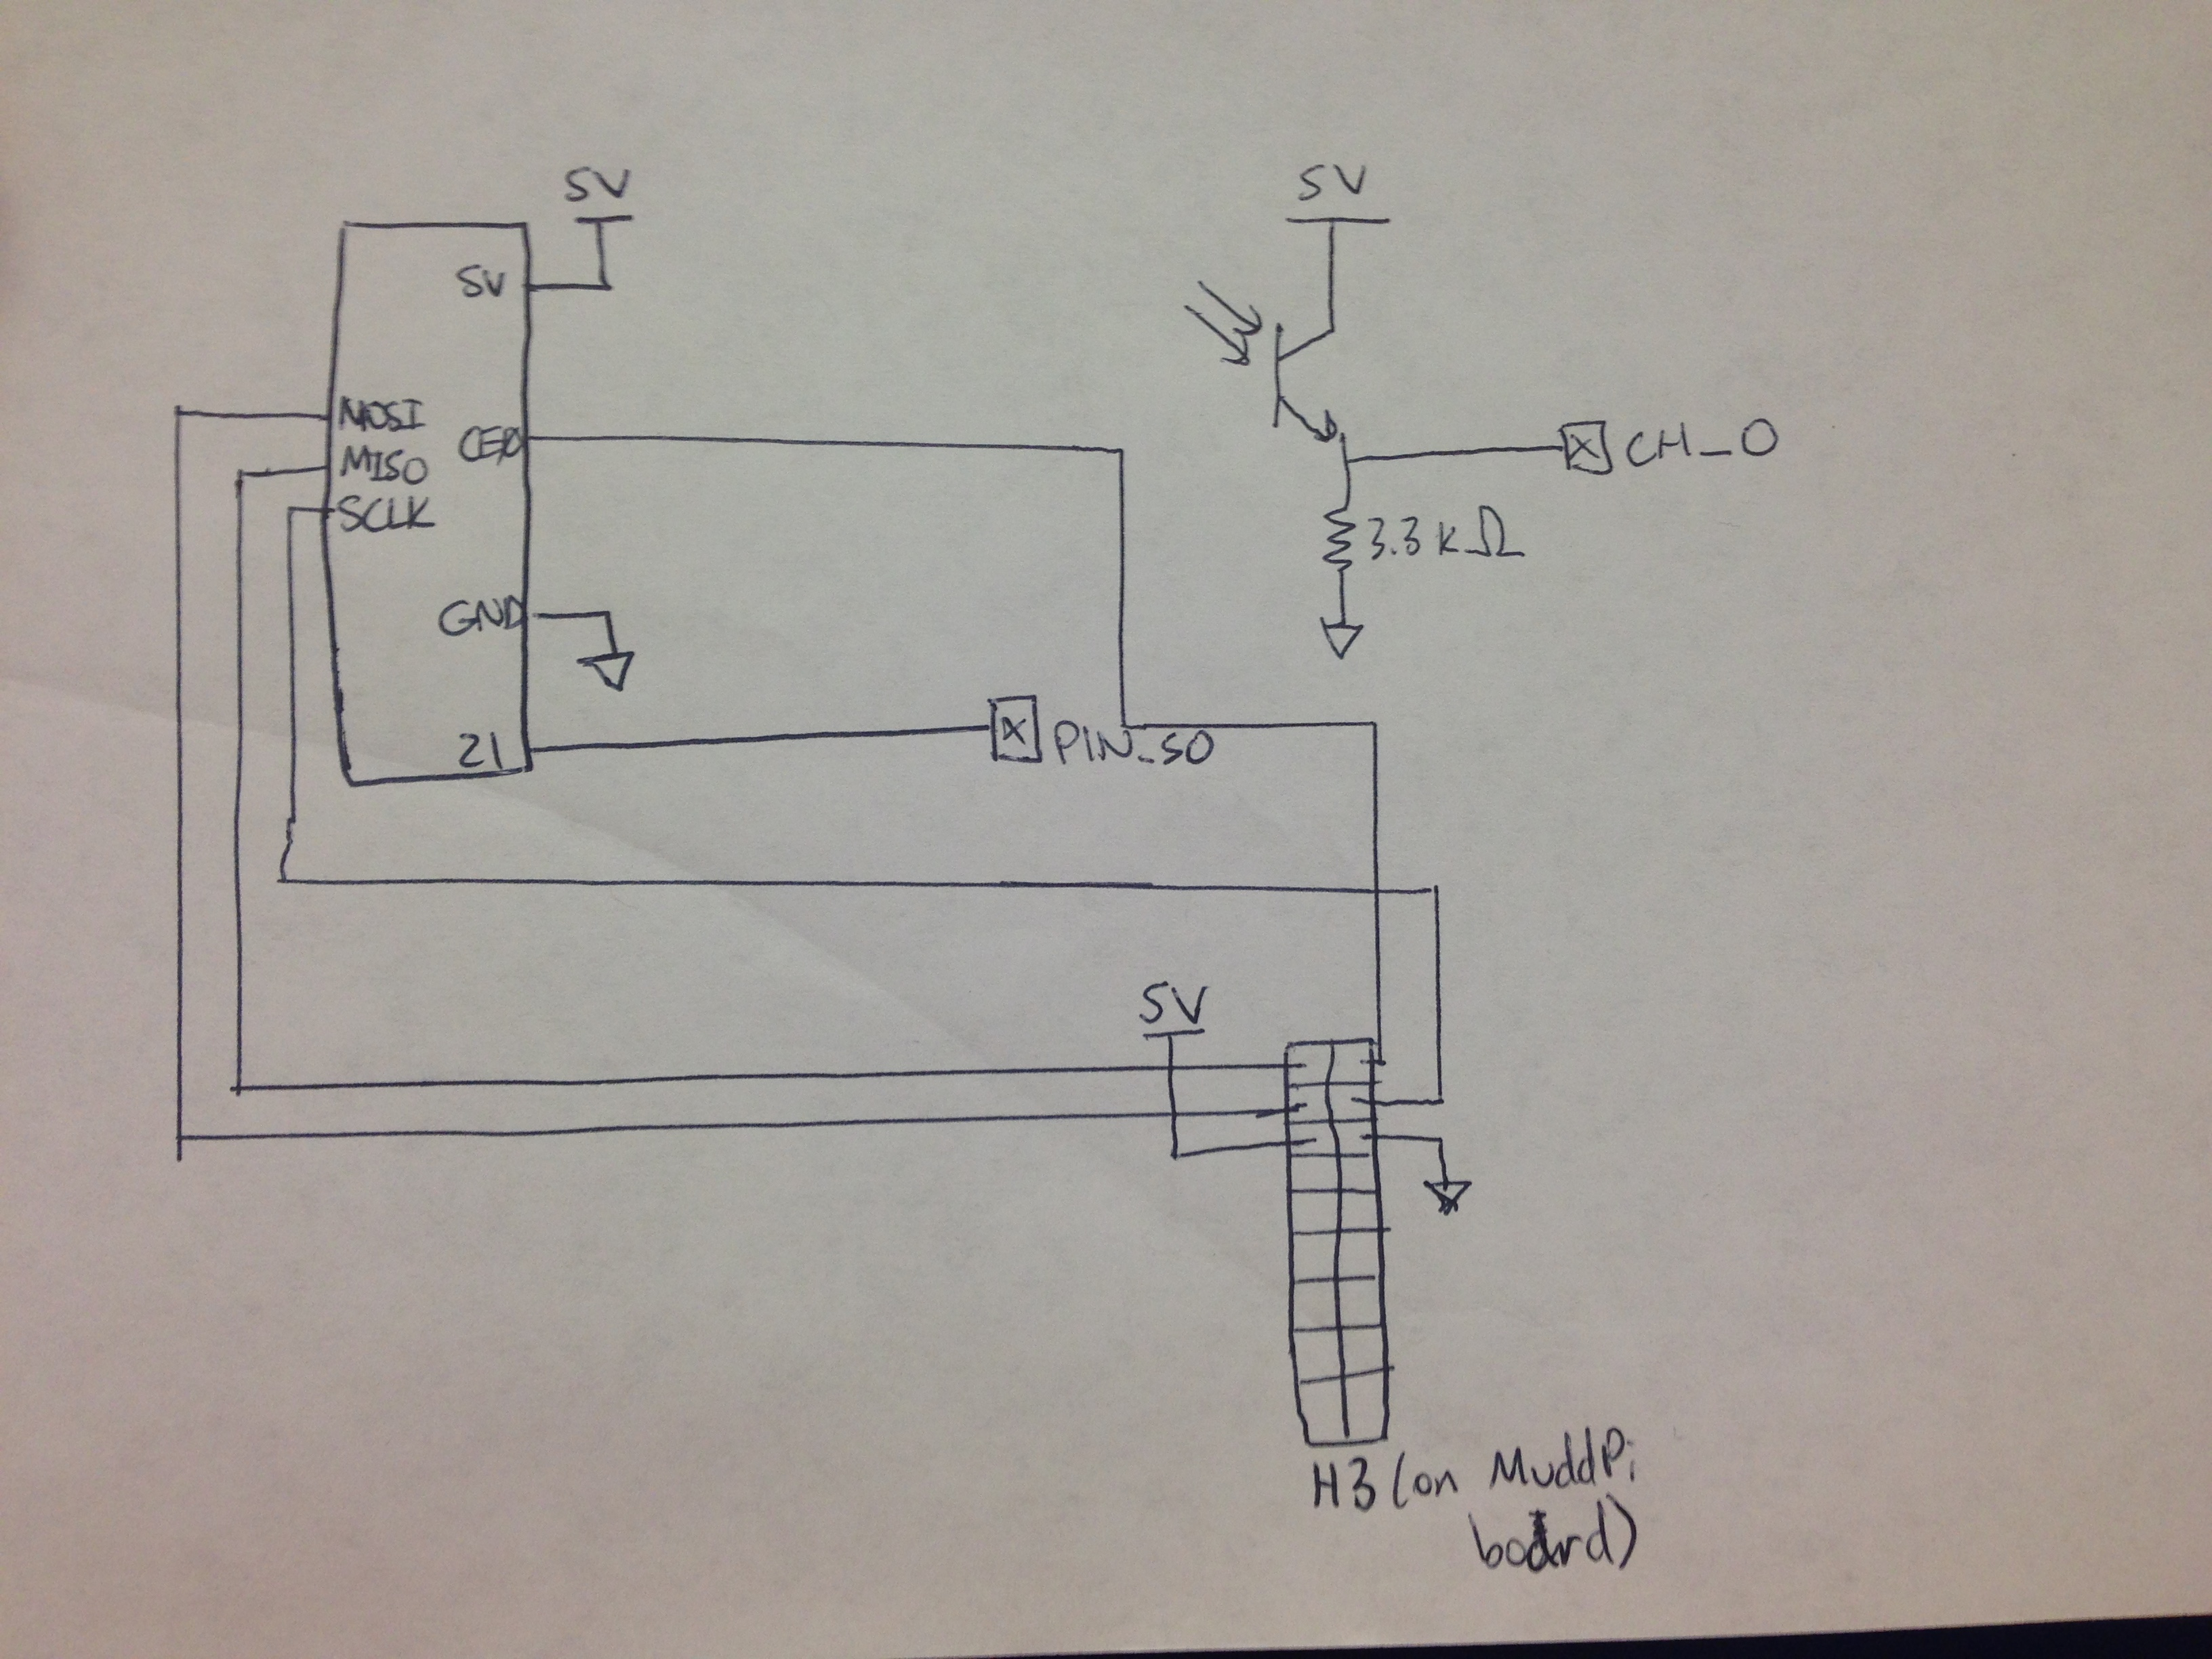
\includegraphics[scale=0.15]{lab6schematic}


\noindent\textbf{C Code}\\
\lstset{language=C}
\noindent\textbf{piHelpers.h}\\
\lstinputlisting{piHelpers.h}
\noindent\textbf{LOADVOLTAGE.c}\\
\lstinputlisting{LOADVOLTAGE.c}
\noindent\textbf{LEDON.c}\\
\lstinputlisting{LEDON.c}
\noindent\textbf{LEDOFF.c}\\
\lstinputlisting{LEDOFF.c}
\noindent\textbf{lab6.sv}\\
\lstinputlisting{lab6.sv}
\end{document}

